\documentclass[10pt,titlepage]{article}
%\usepackage[dvips]{graphics} 
\usepackage{graphicx}
%\usepackage{subfigure}
\usepackage{longtable}
\usepackage{lscape}
\usepackage[pdftex,colorlinks=FALSE]{hyperref}
\setlength{\belowcaptionskip}{0.5cm} % 0.5cm as an example
\raggedbottom
\usepackage[round]{natbib}
\special{papersize=8.5in,11in} \pagestyle{myheadings}
\graphicspath{{figures/}}
\usepackage{fancyhdr}
%\usepackage{fancybox}
%\usepackage{pseudocode}
\pagestyle{fancy}
\lhead{\bf \sc Spherical SOM and Irregular Topology }
\lfoot{Charles R. Schmidt}\rfoot{MS Thesis Proposal}\cfoot{\thepage}
\renewcommand\headrulewidth{1pt}
\renewcommand\footrulewidth{1pt}
\addtolength\oddsidemargin{-2cm}
\addtolength\textwidth{4cm}
\addtolength\headwidth{4cm}
\addtolength\topmargin{-.25in}
\addtolength\textheight{0.25in}
\addtolength\headheight{6pt}
\listfiles
\title{Effects of Irregular Topology in Spherical Self-Organizing Maps}
%\title{Effects of Irregular Topology in Non-Planar SOM Variants}
\author{\sc{Charles R. Schmidt}\\Regional Analysis Laboratory\\Department of Geography\\San Diego State University}
\date{\today}

\begin{document}
%\maketitle
\break
\begin{center}
{\Large{\bf Effects of Irregular Topology in Spherical Self-Organizing Maps}}\\*[3mm]
\end{center}
Charles R. Schmidt\\
MS Candidate\\
Department of Geography\\
San Diego State University\\\\
\today\\\break
Committee Members\\
Dr. Sergio Rey, Geography\\
Dr. Andr{\'e} Skupin, Geography\\
Dr. Robert Malouf, Linguistics\\\break
A Thesis Proposal Presented to the Faculty of San Diego State University.\\
\copyright~2007. Charles R. Schmidt. \\
%% You insert your abstract in the space below.


This document is intended to help students at San Diego State
University to use  \LaTeX\ to produce a Master's Thesis with
high-quality typesetting. Instructions are given for typesetting
complex mathematics and chemical formulas, formatting theorems, using a
variety of table formats, handling figures, and using {\sc Bib}\TeX.  




\\
%\hline
\tableofcontents
\newpage
%\listoffigures
%\newpage
%\listoftables
%\newpage


%
%\documentclass[11pt]{article}
%\setlength{\topmargin}{-.2in}
%\setlength{\oddsidemargin}{-0cm}
%\setlength{\evensidemargin}{-1cm}
%\setlength{\textwidth}{16.3cm}
%\setlength{\textheight}{22.3cm}
%\usepackage{graphicx}
%\usepackage{subfigure}
%\graphicspath{{figures/}}
%\usepackage[round]{natbib}
%\title{Effects of Irregular Topology in Non-Planar SOM Variants}
%\author{\sc{Charles R. Schmidt}\\Regional Analysis Laboratory\\Department of Geography\\San Diego State University}
%\date{\today} %\date{January 29th, 2007}
%\begin{document}
%\maketitle
%\begin{abstract}
%The development of the spherical SOM has been driven by the border effects
%observed in traditional SOM.  Two problems exist with the Spherical SOM. The
%first is the level of control over the network size. The second is the
%topologically induced errors caused by the arrangement of neurons on the sphere.
%Both of these problems stem from the problem of uniformly distributing points on
%a sphere. These problems will be investigated through the introduction of a new
%method for testing topologically induced errors. The method first analyzes  the
%neural network to find topological mis-matches, next we train the network with
%an overwhelming about of synthetic data.  Through a series of simple plots we
%can then compare each neurons internal variance as defined by the variance of
%the observations that best fit that neuron with such metrics as neighborhood
%influence, number of child observations, etc.
%\end{abstract}

\section{Introduction}
The Self-Organizing Map (SOM) is an unsupervised competitive learning process
developed by Teuvo Kohonen as a technique to analyze and visualize high
dimensional data sets.  The applications of SOM are far reaching;
\cite{Kohonen2000} provides a thorough review of the SOM literature including
applications of SOM.  SOM has been used in applications ranging from speech
recognition and image classification to breast cancer detection and gene
expression clustering.  \cite{skupin07} outline the growing interest of SOM in
the GISciences, and propose that the relationship between SOM and GIScience
should be bidirectional.  The SOM is a powerful method for exploring and
visualizing geographic data.  GIScience offers a wide array of tools
and methods to enable the exploration of the SOM itself.  This thesis seeks to 

The SOM is a type of artificial neural network which facilitates the
self-organization of training data onto a network of neurons. The traditional
SOM uses a rectangular or hexagonal network topology \citep{Kohonen2000}.  These topologies 
create a well-known problem in SOM called the boundary effect.  Neurons on
the boundary of the hexagonal and rectangular lattices have fewer neighbors,
which reduces their ability to interact with other neurons during the
self-organizing process.  Using a spherical lattice is widely suggested as a
solution to the problem \citep{ritter99, boudjemai2003, sangole03,
Nishio:2006fk, wu2006}. The use of the spherical lattice, however, does not
completely overcome the boundary problem, and the choice of which spherical
topology to use for the network can be difficult to make.

A regular network topology is one in which every node on the network has the
exact same number of adjacent nodes.  Any topology with an edge is irregular.
Arranging our lattice on the surface of a sphere seems to be an obvious
way to overcome the edge.  However, there exist only five arrangements on the
sphere which are completely regular; these are the five platonic solids \citep{ritter99,
harris2000}.  Any other arrangement of neurons on the surface of the sphere will
result in an irregular topology, as not all neurons will have the same number of
neighbors.  The classic method for minimizing this irregularity is to generate
the spherical lattice by tessellating the sides of the icosahedron
\citep{Nishio:2006fk}.  While this method will always result in a highly
regular spherical topology, the main drawback is that the number of neurons in
the network (the network size), \(N\),
grows exponentially. Other methods for arranging neurons on the sphere allow
for unlimited control over network size, but yield topologies with increased
irregularity \citep{harris2000, wu2005, Nishio:2006fk}.  To date the
literature has largely ignored the more irregular methods in favor of the
aforementioned tessellation-based methods.  A topology which yields a more flexible network
size may be desirable.  However, in order to address this issue of network
size, we must first determine the degree to which irregularity effects the
SOM.

\section{Research Objectives}
The objective of this research is to determine the utility of certain irregular
spherical topologies beyond offering greater control over network size. Toward that
end, I will develop and test new diagnostics to measure and visualize
topology-induced errors in SOM. The following diagnostics
will be developed and implemented:

\begin{enumerate}
    	\item Compare the internal variance of observations captured by a given neuron to that neuron's first-order neighborhood size.
	\item For different topologies, compare the internal variance of each neuron against a composite measure of topological regularity.
	\item Develop a SOM based visualization of the internal variance.
	%\item Develop a reverse quantization error visualization by mapping neurons back onto the input data.
\end{enumerate}

These diagnostics will help facilitate the evaluation of both traditional and
spherical SOMs.  To satisfy the objective of this research, I will apply these
diagnostics to a series of comparable SOMs.  Each SOM will be trained using the
same synthetic data and training parameters, but will utilize different network
topologies.  By formally testing for difference of means and variance in the
results of the diagnostics, the following questions will be addressed:

%topologies.  By formally testing for statistical differences in the
%results of the diagnostics the following questions will be addressed:
\begin{enumerate}
	\item Does the internal variance of a neuron decrease as its first-order neighborhood size, or degree, increases?
	\item Is the average internal variance of a SOM higher when a more irregular topology is used?
	\item Which insights, if any, can be gained from a SOM based visualization of internal variance.
\end{enumerate}

\section{Background}
This section is divided into four parts.  The first provides a general
introduction to the SOM algorithm and the problems created by using irregular
topology. The second reviews the current spherical topologies used with SOMs.
The third examines the flexibility of the various topologies with regard to
network size. The fourth takes a look at the limitations of using ``uniformity''
to evaluate potential topologies.

\subsection{Training and the Boundary Effect}
The SOM algorithm uses an artificial neural network to organize high-dimensional
data onto a low-dimensional lattice, or map, of neurons.  Each neuron contains a
reference vector that models the input data.  Before training, these
neuron-vectors are initialized, most commonly to random values.  During the
training process a randomly selected observation (input vector $x$) searches
each neuron (reference vector $m_i$) to find the one to which it is most
similar, referred to as its Best Matching Unit (BMU $c$).  The BMU and its
neighborhood ($N_c$) are then adjusted to better match that observation
\citep{Kohonen2000}.  The training process is repeated a predefined number of
times, or ideally until the map converges.  The traditional SOM is laid out on a
two-dimensional plane using either a rectangular or hexagonal topology.
According to \cite{wu2006}, the hexagonal structure is more uniform and generally
preferred.

One drawback of building the neural lattice in a discrete Euclidean plane is the
boundary of the resulting lattice.  A neuron located on the boundary has fewer
neighbors and thus fewer chances of being updated \citep{wu2006}.  As observed
in Figure \ref{figure1}, neurons in the center of the map tend to better
represent the mean of the input-space.  This is arguably caused by outliers
being pushed to the edges of the map, where they encounter fewer competing
signals.

\begin{figure}
\centering
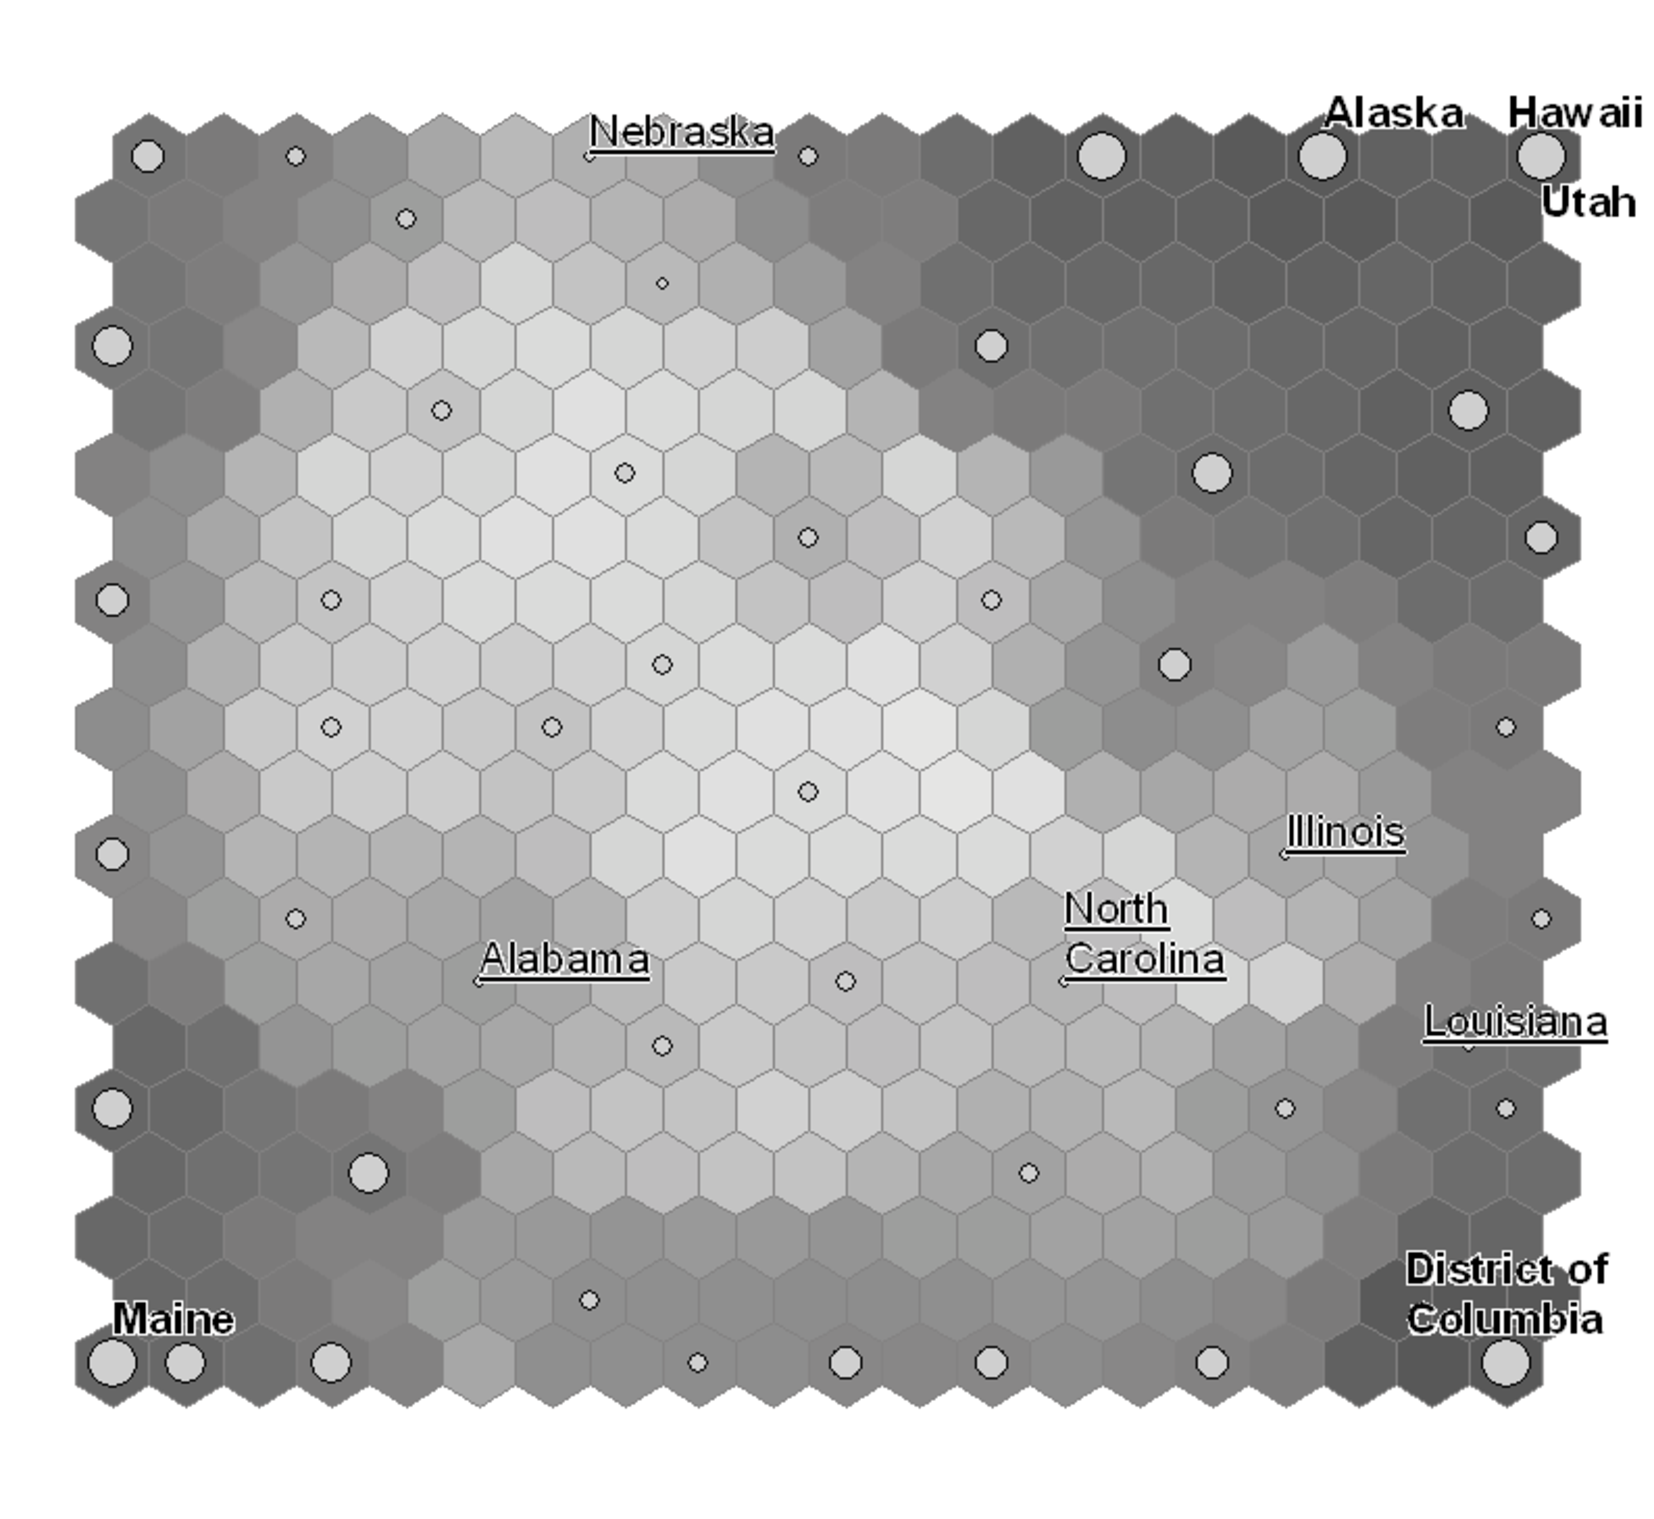
\includegraphics[width=\linewidth]{gridedge_grey.pdf}
\caption{The fifty United States and The District of Columbia mapped onto a
SOM trained with the first thirty-two census variables.  Darker neurons have a
relatively larger difference from the mean of the states, while lighter
neurons are relatively closer.  Smaller dots show states that are closer to the
mean, while large dots show outliers. The five most average states are shown
with underlined labels and the five states furthest from the mean are shown with
bold labels.}
\label{figure1}
\end{figure}


\subsection{Spherical SOM}
One way to eliminate the boundary effect is to wrap the lattice around a
three-dimensional object such as a sphere or torus, thereby removing the edge
entirely. The toroidal SOM was introduced by \cite{li1993}, however the torus is
not effective for visualization, as maps generated from a torus are not
very intuitive \citep{ito2000,wu2006}.  \cite{ritter99} describes the torus as
being topologically flat and suggests that a curved topology, such as that of a
sphere, may better reflect directional data.  A sphere also results in a more
intuitive map, since we are accustomed to looking at maps based on a sphere.

\cite{ritter99} first introduced the spherical SOM, and several enhancements have
since been suggested \citep{boudjemai2003,sangole03,Nishio:2006fk,wu2006}.  A
good comparison of these enhancements can be found in \cite{wu2006}.  All of
these methods derive their spherical structure through the tessellation of a
polyhedron as originally proposed by \cite{ritter99}.  \cite{wu2006} point
out the importance of a uniform distribution on the sphere, and that it is
preferable for all neurons to have an equal number of neighbors and to be
equally spaced.  They find generally that the tessellation method best satisfies
these conditions, and specifically that the icosahedron is the best starting
point \citep{wu2005}. Tessellation of the icosahedron results in a network of
neurons, each of which have exactly six neighbors, save the original twelve
which each have five.  This is very close to the ideal structure in which every
neuron would have exactly six neighbors.  This structure has very low variances
in both neuron spacing and neighborhood size.

\subsection{Network Size}
\begin{figure}
\centering
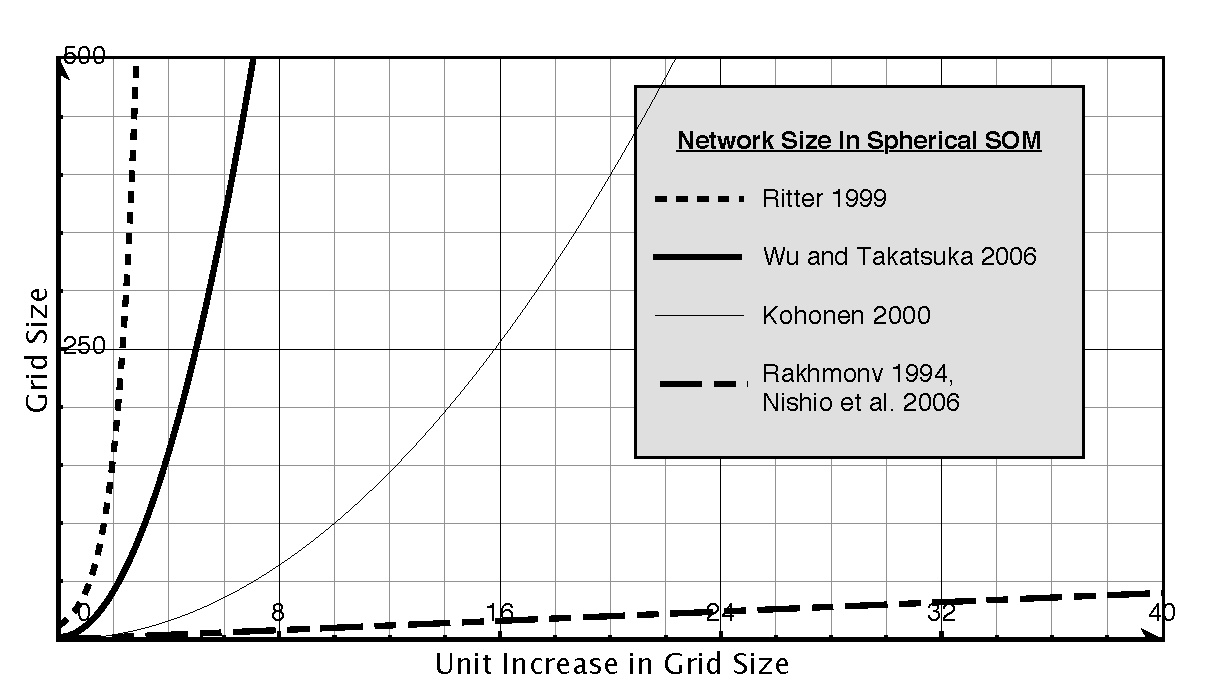
\includegraphics[width=\linewidth]{networkSize.pdf}
\caption{This figure demonstrates the achievable network size using various
spherical topologies. The Y-axis represents the achievable network size, the
meaning of the X-axis is dependent on the topology. For the tessellation
methods the X-axis represents the frequency of the tessellation. For the
traditional Kohonen methods the X-axis represents the size of both dimensions of
the grid, for comparability the ratio between the dimensions was fixed at one
($X_{dim}=Y_{dim}$).  For the \cite{Rakhmanov94} and \cite{Nishio:2006fk} methods the X-axis
represents the exact network size.}
\label{fig:nSize}
\end{figure}
The literature offers little theoretical guidance on network size
\citep{cho1996}.  \cite{toolbox} suggests simply using a network size of
\(5\sqrt {n}\), where \(n\) is the number of observations. Given this lack of
theoretical development, researchers should be cautious when using methods that
limit the control of network size.  As shown in Figure \ref{fig:nSize},
methods for arranging an arbitrary number of points on a sphere provide a much
higher degree of flexibility when choosing a network size.

The cost of relying on \citeauthor{ritter99}'s tessellation method is decreased
control over network size. \citeauthor{ritter99}'s tessellation method results
in a network size that grows at a rate of \(N=2+10*4^f\), where $f$ is the
frequency of tessellation. \cite{wu2006} offer a slight improvement. Rather than
recursively subdividing the faces, they redivide the original icosahedron with
each step, resulting in \(N=2+10*f^2\).  In practice 2D Euclidean SOMs also offer
limited control over network size because it is undesirable to have one dimension
dramatically larger than the other. \cite{Nishio:2006fk} try to address the
issue of network size granularity by departing from the tessellation method and
suggesting the use of a partitioned helix to uniformly distribute any number of
neurons on a sphere.  A similar method proposed by \cite{Rakhmanov94} was
dismissed by \cite{wu2005} for failing to satisfy the uniformity conditions
described above.

\subsection{Uniformity}
\citeauthor{wu2006} state that ``[f]or SOM, it is desirable to have all neurons
receive equal geometrical treatment'' \cite[p. 900]{wu2006}.  To satisfy this
constraint, two conditions must be met.  First, each neuron should occupy the
same amount of space on the given surface.  Second, each neuron should be
bordered by the same number of surrounding neurons, and we should maximize that
number.  The first condition is important for visualization, but
irrelevant for training.  During the training of the SOM only the topology of
the neurons is considered.

Based solely on measures of neuron spacing, \cite{wu2005} dismissed a method
proposed by \cite{Rakhmanov94} for distributing points on a sphere.  Similarly
\cite{Nishio:2006fk} use these variance measures to support their helix
algorithm for distributing points on a sphere.  Table \ref{table1} shows that
these metrics can be misleading and may not be comparable across topologies.
The traditional rectangular and hexagonal topologies have no variance in neuron
spacing, and the generally preferred hexagonal structure displays greater
variance in neighborhood size than the rectangular structure.  The torus, by
comparison, would have variance in neuron spacing, yet no variance in
neighborhood size.  The distance between two neurons is only considered during
the formation of the neural network.  At this stage the spacing is significant
as it plays a part in determining neuron adjacency. However, using this measure
to evaluate potential topologies for use in SOM may be misleading.

\begin{table}[htbp]
\caption{Variances in Topologies}
\begin{center}
\begin{tabular}{|c|c|c|c|}
\hline
Topology&Grid Size&Neuron Spacing&Variance in Neighborhood Size\\
\hline
Rectangular&9x18&1&0.2716\\
Hexagonal&9x18&1&1.2138\\
Tessellation&162&0.25319 - 0.31287& 0.0686\\
Rakhmanov&162&0.15779 - 0.30069& 0.2908\\
\hline
\end{tabular}
\end{center}
\label{table1}
\end{table}

Methods for distributing points on the sphere, which allow for fine-grained
control over network size, produce slightly more irregular topologies.  However,
no substantive discussion of these irregularities or their effects on SOM
training exists in the literature. Given that limited theoretical guidance is available
for choosing network size, the desire for finer control over the network size
should not be overlooked. Particularly for larger SOMs, the desired network size
may not be achievable via tessellation of the icosahedron.

\section{Data and Methodology}
This section is composed of two parts.  The first describes the diagnostics
developed for evaluating network topologies.  The second describes an
empirical study that will implement these methods in order to evaluate the
utility of new and/or unfashionable topologies.

\subsection{Diagnostics}
Three diagnostics are developed to explore the effect of irregular topology on
spherical SOM.  The first diagnostic will be used to address the research
question regarding the internal variance and neighborhood size.  The second
diagnostic will address the question concerning internal variance and
topological irregularity.  The third tool will help visualize the patterns
between internal variance and topology.

\subsubsection{Internal variance vs. first-order neighborhood size}
This diagnostic will compare the internal variance of each neuron against its
first-order neighborhood size.  In traditional SOMs, outlying observations are
pushed to the edge of the map where they encounter fewer competing signals. A
prime example of this is the ``Utah-Hawaii'' case shown in Figure
\ref{figure1}.  Relying only on the SOM, one would be left to believe that the
two states are similar. Upon closer inspection we see that the QError from
Utah to the neuron is $1.509$, the QError from Hawaii to the neuron in
$1.505$, but the QError from Utah to Hawaii is $3.014$. In this case only Utah
and Hawaii were mapped to that neuron.  In a case where multiple observations
land on the same neuron, it is possible to measure average pairwise QErrors
between those observations.  This gives us a notion of internal variance for
each neuron. It would be expected that in traditional SOMs neurons closer to
the edge will have higher internal variances. This can be extended to
spherical SOMs by comparing the degree of a neuron ($deg(m_i)$ or the number of
adjacent neurons) to its internal variance.

Once the internal variance ($var(m_i)$) and degree ($deg(m_i)$) of each neuron
have been calculated, the neurons can be separated into a small number of
groups based on the degree \footnote{For most topologies the number of
different degrees will be limited to three or four.}.  The variance and mean
will be calculated for each of these groups.  The expected result is that
variances and means of the groups will decrease as the degree increases.  This
hypothesis will be tested using a ratio of variances test and a difference of
means test.  The result will also be visualized using a box plot.

\subsubsection{Internal variance vs. topological regularity}
This diagnostic will compare the internal variance of each neuron against a
measure of regularity for its associated topology.  The degree of each neuron
can easily be calculated by taking the column sums of the first-order
adjacency matrix ($A$).  A completely regular network topology (i.e. the
torus) will have no variance between these column sums.  For irregular
networks the variance between these column sums gives us a measure of
irregularity. There are many alternative ways to classify the connectivity of
a network; \cite{florax95} outline four such summary measures, which will be
evaluated for use in this diagnostic.  For each topology we can compare the
internal variances as described above against a measure that summarizes the
given topology's regularity.

This diagnostic is evaluated in much the same way as the last diagnostic.  
The internal variances are this time grouped by their topology.  We can then
compare the variances of internal variances and the means of the internal
variances across topologies.  It is expected that the distribution of internal
variances will be narrower for groups trained on more regular topologies.
It is further hypothesized that the means of these internal variances will
decrease with more regularity.  These assumptions will be tested using
a \emph{t-test} on the means and an \emph{F-test} on the variances.

\subsubsection{Visualize internal variance mapping}
Visualizing the internal variance may yield insight into how irregular topology
effects the SOM.  Once the internal variance of each neuron has been calculated
we can use the values to color or shade a map of the given topology.  The degree
to the neurons can be visualized using proportional symbols to help show
patterns between internal variance and irregularity.

\subsection{Empirical Analysis}
The empirical analysis consists of three main tasks.  The first is to create
synthetic data suitable for the diagnostics described above.  The second task is
to train multiple SOMs, each of with a different topology type. The third task
will be to apply the diagnostics and interpret the results.

\subsubsection{Synthetic Data}
In order to test the methods described above, I will generate high-dimensional
synthetic data with known properties.  Knowing the properties of the training
data allow us to systematically compare the diagnostics under several different
topologies.  To ensure that we can calculate an internal variance for each
neuron, I will generate the data so as to increase the probability that each
neuron will be occupied by more than one observation.
\subsubsection{Training}
The diagnostics must be given a trained SOM for each topology to be compared. To
yield any meaningful results those SOMs must be trained with comparable
parameters. Most parameters can simply be set to the same value for each SOM.
However, special consideration must be given to network size.  As shown in
Figure \ref{fig:nSize}, topologies differ in terms of achievable network size.
This analysis will include the following topologies:
\begin{itemize}
\item Rectangular
\item Hexagonal
\item A topology based off \cite{Rakhmanov94}
\item The Helix topology proposed by \cite{Nishio:2006fk}\footnote{Currently
there is some uncertainty about the ability to include the Geodesic and Helix
type topologies given the complexities involved with their implementation.
However, an additional goal of this project to provide a framework on which new
topologies can be easily implemented and tested by future researchers.}
\item The Geodesic topology proposed by \cite{wu2006}\footnotemark[2]
\end{itemize}

\subsubsection{Diagnostics}
The first diagnostic will yield a set of results for each topology test.  These
results will be analyzed in order to address the first research question of this
paper.  The second diagnostic provides one set of results.  These results will
be analyzed to address the second research question.  The final diagnostic will
return a visualization for each topology tested.  The usefulness of these
visualizations is a research question in itself.  The expectation is that the
visualizations will show patterns of internal variance related to irregularities
in the network topology.

\section{Significance and Limitations}
\subsection{Significance}
The commonly used tessellated icosahedron based topology offers a near ideal
base for spherical SOMs.  The main disadvantage of this topology type is that it
offers a limited control over network size.  Alternative methods for generating
the spherical topology, which can create a network of any size, have been
reviewed or suggested by \cite{wu2005} and \cite{Nishio:2006fk}.  These
alternative methods produce network structures that are more irregular.  This
research will take a closer look at the impact that the irregularity has on the
training process in an attempt to address the suitability of these topologies
for use in SOM.

\subsection{Limitations}
This research will look at the relationship between regularity in neuron connectedness
and the training of a SOM. The relationship between topology and SOM visualization is not
addressed. The topology chosen for a SOM has a direct link with how that SOM is
visualized.  When representing the topology on the surface of a sphere issues
arise with the uniformity in neuron spacing and sizing.  Future work may be
needed to address these issues in visualization.

%\subsubsection{Synthetic Data} I will take advantage of weights matrices to generate synthetic training data with known properties.  This data will be used to train the various SOMs in order to facilitate comparison.

%\subsubsection{Train SOM}

%It is useful to represent our neural lattice as a graph, G.
%We know that any arrangement of neurons onto the surface of a sphere will as such the network can be effectively treated as a graph.  Doing so enables us to use the properties of the graph and the principles of graph theory to help us understand the relationship between neurons during training.

%the variance in neuron spacing should be minimized.    The first condition ensures that each neuron will occupy is only of concern when visualizing the SOM.

%The get at the second condition we must first define the degree of a neuron, deg(n) to be number of its direct neighbors.  Whit that in mind the second condition is that the variance in the degree of the neurons must also be minimized.

%This statement may be somewhat misleading to those investigating alternative 

%For the purpose of SOM visualization it is important for each neuron to receive equal geometrical treatment.

%It is useful to represent the neural network as a graph, G, in order use the...
%In order to examine the irregularities in the neural network it is useful ....

%The basic problem of the "boundary effect" is that neurons on the edge have fewer neighbors. Yet there are only five possible arrangements of points on a sphere such that all points have the same number of neighbors.  Any spherical lattice consisting of more then twenty (dodecahedron) neurons will contain topological irregularities.  This is to say that not all neurons will have the same number of neighbors.  The importance of these irregularities and the magnitude of their effects on SOM training is not known.  This goal of this research is to determine whether more flexible network structures may be used in spherical in SOM without introducing significant errors. To accomplish this goal, basic methods in network analysis with be combined with the result from several empirical training runs each utilized different topology.  

\bibliographystyle{apalike}
\bibliography{som}
\end{document}
